\documentclass[11pt]{paper}

\usepackage[T1]{fontenc}

\usepackage{graphicx}
\usepackage{amssymb}
\usepackage{amstext}
\usepackage{amsmath}
\usepackage{a4wide,color}
\usepackage[utf8]{inputenc}
\usepackage[frenchb]{babel}
\usepackage{xspace}
\usepackage{anysize}
\usepackage{tabularx}
\usepackage{multirow}
\usepackage{fancybox}
\usepackage{fancyhdr}
\usepackage{bbding}

\usepackage{caption}
\usepackage{subcaption}


\usepackage{color}
\usepackage{float}

\usepackage[toc,page]{appendix} 
\usepackage{lscape}

\usepackage{placeins}

\usepackage{listings}
\lstdefinestyle{customc}{
  belowcaptionskip=1\baselineskip,
  breaklines=true,
  frame=L,
  xleftmargin=\parindent,
  language=C,
  showstringspaces=false,
  basicstyle=\tiny\ttfamily,
  keywordstyle=\bfseries\color{green!40!black},
  commentstyle=\itshape\color{purple!40!black},
  identifierstyle=\color{blue},
  stringstyle=\color{orange},
  tabsize=2
}

\usepackage{todonotes}

\usepackage[framemethod=TikZ]{mdframed}

\lstset{% general command to set parameter(s)
	basicstyle=\footnotesize, % print whole listing small
	keywordstyle=\color{magenta}\bfseries, % underlined bold black keywords
	identifierstyle=, % nothing happens
	commentstyle=\color{black}, % white comments
	stringstyle=\ttfamily, % typewriter type for strings
	showstringspaces=false % no special string spaces
} 

\lstdefinelanguage{aald}
	{morekeywords={system, implementation},
	sensitive=false,
	morecomment=[l]{//},
	morecomment=[s]{/*}{*/},
	morestring=[b]",
}

\usepackage[colorlinks=true]{hyperref}

\usepackage[normalem]{ulem}
\usepackage{color}

\definecolor{Fond}{gray}{0.7}

\renewcommand{\floatpagefraction}{.99}
\renewcommand{\textfraction}{.01}
\newcommand{\modif}[1]{\textcolor{red}{\uline{#1}}}


\pagestyle{fancy}
\fancyhf{}
\fancyhead[RE,RO]{\thepage}
\fancyhead[LE]{}
\fancyhead[LO]{Temps réel }
\fancyfoot[LO]{Centrale Nantes -- \today}
\fancypagestyle{plain}{%
  \fancyhf{} % get rid of headers
  \renewcommand{\headrulewidth}{0pt} % and the line
}

\newenvironment{maliste}%
{ \begin{list}%
	{\ArrowBoldRightStrobe}%
	{\setlength{\labelwidth}{30pt}%
	 \setlength{\leftmargin}{35pt}%
	 \setlength{\itemsep}{\parsep}}}%
{ \end{list} }

 \setlength{\parskip}{1.2ex plus .9ex minus .4ex}

\newcommand{\ocv}{{\tt OpenCV}\xspace} 
\newcommand{\alsa}{{\tt ALSA}\xspace} 
\newcommand{\aadl}{{\tt AADL}\xspace} 
\newcommand{\xeno}{{\tt Xenomai}\xspace} 
\newcommand{\iic}{I$^2$C\xspace} 


\title{{\Large Systèmes interconnectés -- SINT }\\
\vspace{-0.4em}
{\large Sujet de TP 4 : CAN}\\
{\small Centrale Nantes}\\
\small P.-E. Hladik, \small{\texttt{pehladik@ec-nantes.fr}}\\
---\\
{\scriptsize  Version bêta (\today)}\\
}


\begin{document}

\maketitle

%\begin{table}[htdp]
%\caption{Suivi des modifications}
%\begin{center}
%\begin{tabular}{|c|c|c|p{8cm}|}
%\hline
%Date & Version & Auteur & Modifications\\
%\hline
%JJ/MM/12 & 0.3.X & P.-E. Hladik&  \\
%\hline
%\end{tabular}
%\end{center}
%\label{default}
%\end{table}%

%%%%%%%%%%%%%%%%%%%%%%%%%
  \section{Objectifs pédagogiques}
%%%%%%%%%%%%%%%%%%%%%%%%%


\begin{itemize}
	\item mettre en œuvre un échange de messages sur un bus CAN
	\item observer et comprendre le bit stuffing et l'arbitrage de priorité
	\item estimer les temps de transition d'un message CAN
\end{itemize}

%%%%%%%%%%%%%%%%%%%%%%%%%
  \section{Rendu}
%%%%%%%%%%%%%%%%%%%%%%%%%

Le travail est prévu pour deux séances de TP. À la fin, déposez sur Hippocampus une archive avec un (petit) compte rendu en pdf et les extraits de code pertinents.


%%%%%%%%%%%%%%%%%%%%%%%%%
  \section{Mise en œuvre d'une communication sur un bus CAN}
%%%%%%%%%%%%%%%%%%%%%%%%%

Vous allez utiliser les cartes Feather M0 et Teensys pour mettre en œuvre une communication sur le bus CAN à l'aide des bibliothèques Arduino.

\subsection{Envoi et réception d'un message sur le CAN}
\label{sec:leds}

Le premier objectif est de faire changer l'état de la led L[x] (x=0..2) de la carte Teensy 3.6 suite à l'appuie sur le bouton poussoir P[x] (x=0..2) de la carte Feather M0 (voir figure~\ref{fig:ds_led}). Le schematic de la carte teensys peut être trouvé sur \href{https://github.com/pierremolinaro/cartes-micro-controleurs-centrale-nantes/blob/master/carte-teensy-3-6/schematics.pdf}{schematics.pdf}. Mais d'ailleurs sur quelle broche est connecté le CAN ?

\begin{figure}[htbp]
\begin{center}
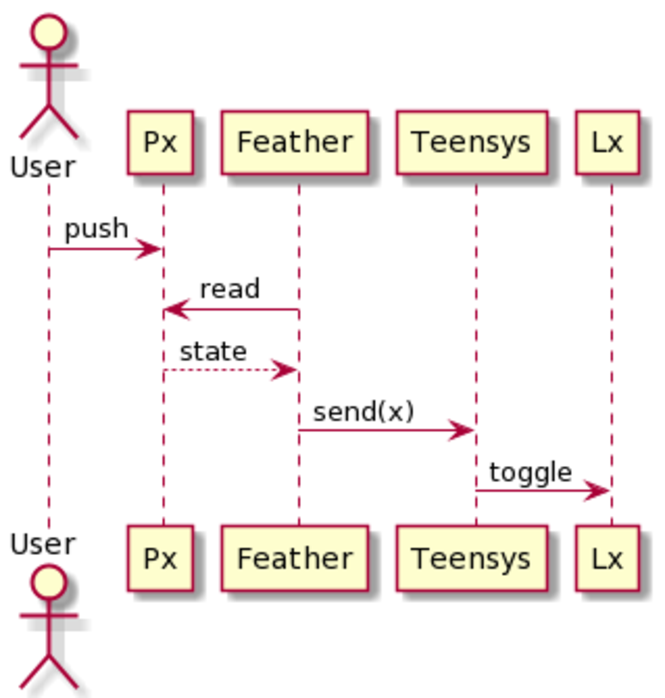
\includegraphics[scale=0.5]{./figures-pdf/diag_seq_led}
\caption{Diagramme de séquence pour le contrôle des leds}
\label{fig:ds_led}
\end{center}
\end{figure}


%@startuml
%
%actor User
%
%
%User -> Px : push
%Feather -> Px : read
%Px --> Feather : state
%Feather -> Teensys : send(x)
%Teensys -> Lx : toggle
%
%@enduml

\paragraph{Installation des librairies.} Pour ce TP vous utiliserez les libraires ACAN pour le Teensys et ACAN2515 pour la Feather.% Ce TP s’effectue sur la carte Teensy 3.6. Le plus simple est de partir du croquis LoopBackDemo, qui est parmi les exemples de la librairie. Pas de compte-rendu pour ce TP.

Commencez par télécharger la dernière version de la librairie ACAN à partir de l'environnement Arduino (menu Croquis > Inclure une bibliothèque > Gérer les bibliothèques). Faites de même pour la librairie ACAN2515. %à partir de l'environnement Arduino, et partez du croquis d'exemple LoopBackDemoAdafruitFeatherM0.

Les bibliothèques ACAN et ACAN2515 contiennent les fichiers source qui seront compilés, la documentation en PDF (à consulter pour faire ce TP) et des croquis d'exemple, dont LoopBackDemo et LoopBackDemoAdafruitFeatherM0 qui peuvent vous servir de base comme exemple (les versions avec filtre peuvent être aussi utiles).

Pour ouvrir les croquis d'exemple LoopBackDemo et LoopBackDemoAdafruitFeatherM0 aller dans le menu Fichier > Exemples > ACAN > LoopBackDemo ou Fichier > Exemples > ACAN2515 > LoopBackDemoAdafruitFeatherM0.

\paragraph{Test et mise au point.} Afin de mettre au point votre application, vous pouvez facilement réaliser des tests en mode LoopBack.

\paragraph{Contraintes.} Vous devez utiliser les filtres de réception.

\paragraph{Conception.} C'est à vous de définir les messages : identificateur, structuration de l'information, etc. Indiquez dans le rapport le format des vos messages.

\paragraph{Conseils.} Vérifier que les interrupteurs de terminaison sont activés sur les interfaces.


\subsection{Mise en place d'une communication de type requête-réponse}

Le second travail consistera à mettre en place un système pour afficher sur la Teensys l'état du codeur incrémental de la Feather suite à l'appui du boutons P0 sur la Teensys. Proposer une solution avec un mécanisme de type {\it Request–reply} (figure~\ref{fig:rr_pattern}) et un second avec une publication périodique de l'état du codeur incrémental (figure~\ref{fig:periodic}).

\begin{figure}[htbp]
\begin{center}
	\begin{subfigure}[b]{0.45\textwidth}
        		\centering
		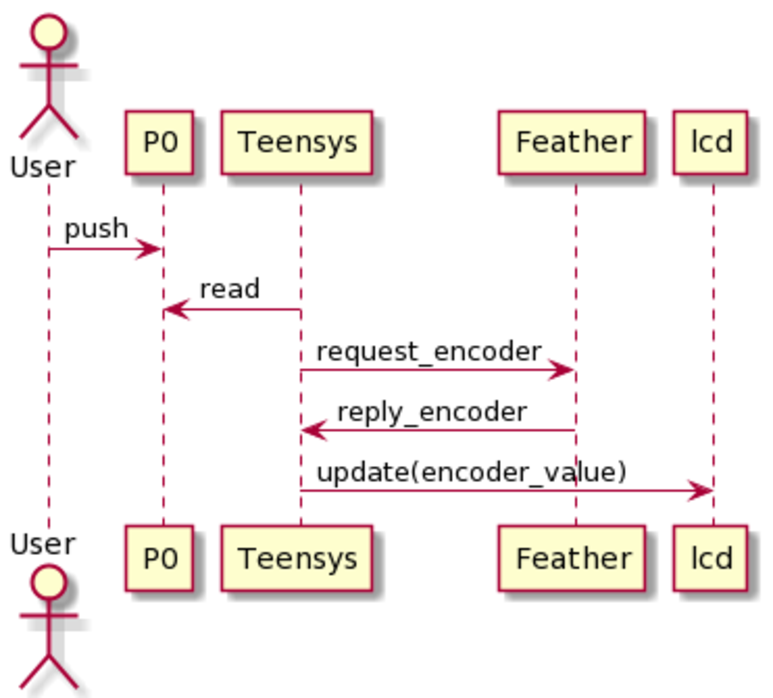
\includegraphics[width=\textwidth]{./figures-pdf/request_reply}
         	\caption{{\it Request-Reply} pattern}
         	\label{fig:rr_pattern}
	\end{subfigure}
	\begin{subfigure}[b]{0.45\textwidth}
        		\centering
		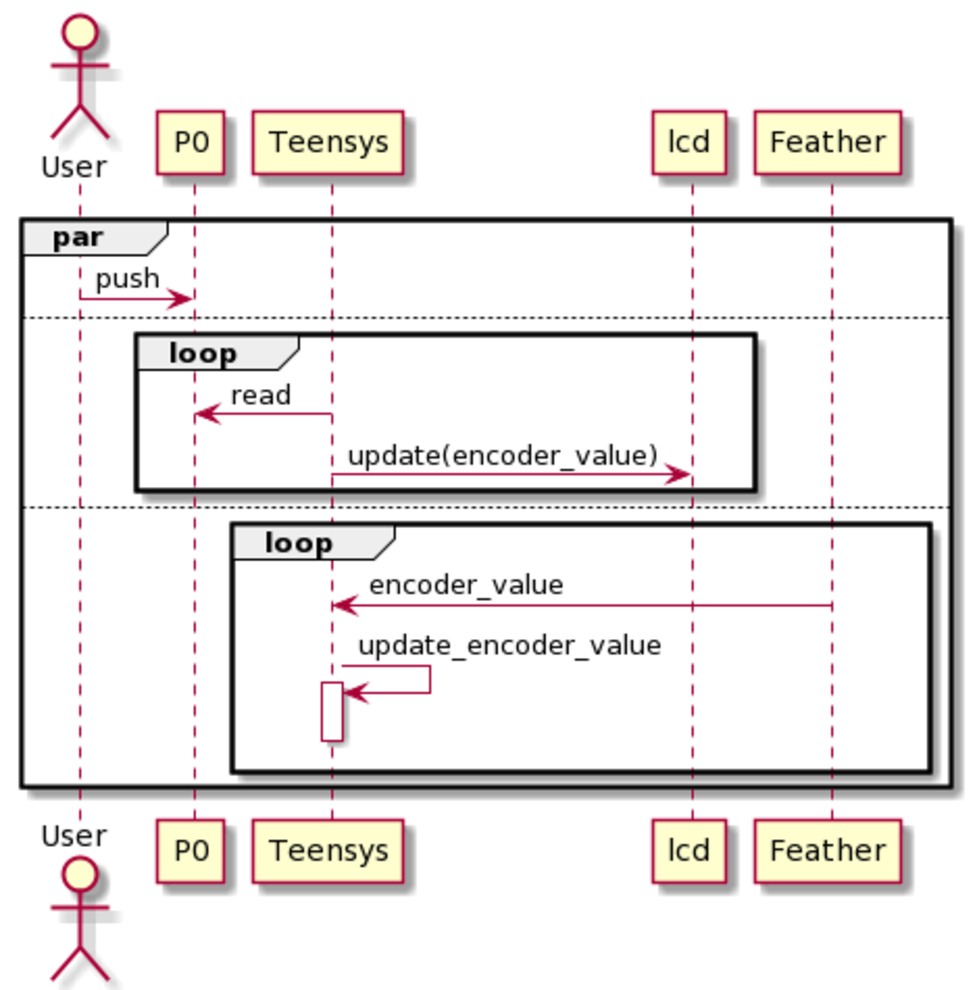
\includegraphics[width=\textwidth]{./figures-pdf/periodic}
         	\caption{Pattern periodique}
         	\label{fig:periodic}
	\end{subfigure}
\end{center}
\caption{Patterns d'échange de données}
\end{figure}

%@startuml
%
%actor User
%
%
%User -> P0 : push
%Teensys -> P0 : read
%Teensys -> Feather : request_encoder
%Feather -> Teensys : reply_encoder
%Teensys -> lcd : update(encoder_value)
%
%@enduml

%@startuml
%
%actor User
%
%par
%User -> P0 : push
%else
%  loop
%    Teensys -> P0 : read
%    Teensys -> lcd : update(encoder_value)
%  end
%else
%loop
%  Feather -> Teensys : encoder_value
%  Teensys -> Teensys : update_encoder_value
%  activate Teensys
%  deactivate Teensys
%end
%end
%@enduml

Pour chacune des solutions, mesurer le temps de réaction entre l'appui sur le bouton et l'affichage, ainsi que la fraîcheur de la valeur. Pour faire ces mesures, programmer des broches sur les cartes pour générer des signaux permettant de mesurer les temps et utiliser l'analyseur pour relever ces informations.

Si on voulait faire un affichage périodique de la valeur du codeur de la Feather sur la Teensys quelle solution vous semblerait la plus appropriée ? Expliquez dans le rapport pourquoi.


%%%%%%%%%%%%%%%%%%%%%%%%%%
\section{Bit-stuffing, arbitrage et détection d'erreur}
%%%%%%%%%%%%%%%%%%%%%%%%%%

Connecter la Teensy 3.6 à la STM32. La liaison CAN se fera entre le CAN0 de la Teensy 3.6 et la carte STM32 (qui n’a qu’un module CAN).
Vous avez les broches TX et RX du CAN de la STM32 (entre le transceiver et le $\mu$C) qui sont accessibles pour connecter un analyseur logique (le schéma de la petite carte STM32 est sur Hippocampus).

\subsection{Observation du bit-stuffing}

Envoyer une trame de données standard, dont l'identificateur est 0x110, qui contient 2 octets de données (0x10 et 0x34 par exemple). La carte STM32 doit répondre avec une autre trame de donnée.

Quelle est l’identifiant de cette trame? Comment ont été modifiées les données (il faudra certainement faire plusieurs essais avec des données différentes)? Expliquer les différences entre les broches RX et TX (lors de l’envoi et de la réception d’une trame par le nœud STM32). Pour les données 0x10 et 0x34, combien de bits sont rajoutés (bit stuffing)?

\subsection{Identification d'une trame}

Il y a 4 interrupteurs et 2 boutons poussoirs sur la carte STM32. On n’utilisera pas encore le bouton poussoir (PA1) le plus proche du connecteur CAN ! On sait que la modification d’un des 4 interrupteurs, ou l’appui sur le bouton poussoir (PA0) génère l’envoi d’une trame standard de 1 octet, mais l’identifiant a été perdu! On sait uniquement qu’il se situe entre 0x200 et 0x300.

Déterminer l’identifiant associé et le protocole utilisé (même principe que pour la partie liaison série). Programmer une application basique tel que chaque interrupteur allume une led différente de la teensy3.6

\subsection{Identification d'une trame (bis)}

Il y a 4 leds sur la carte STM32. On sait que ces leds sont pilotées par une trame standard de 1 octet, mais l’identifiant a aussi été perdu! On sait uniquement qu’il se situe entre 0x10 et 0x100.

Déterminer l’identifiant associé et le protocole utilisé (même principe que pour la partie liaison série). Les LEDs L0 à L3 sont respectivement connectées sur les broches D12, D11, D3 et D6 de la carte STM32.

\subsection{Trame d'erreur}

L’appui sur le bouton poussoir (PA1) à côté du connecteur CAN provoque l’envoi d’une trame avec une erreur sur le bus. Pour forcer cette erreur, le nœud commence une transmission CAN, puis passé un court délai reconfigure la broche de transmission en I/O sur un court laps de temps pour générer une erreur. La broche D9 est mise à 1 pendant ce laps de temps.

Expliquer le comportement (analyseur logique): Quel est le déroulement chronologique? Qu’est ce qui a été modifié sur la trame? Quelle est l’erreur associée? Comment réagissent les autres nœuds? Quel est la durée totale de cette gestion d’erreur sur le bus?

Attention: le décodeur de protocole n’est pas capable de détecter une erreur (fonction non implémentée). Il sera nécessaire de regarder directement la trame binaire!

%%%%%%%%%%%%%%%%%%%%%%%%%%
\section{Application à trois partenaires}
%%%%%%%%%%%%%%%%%%%%%%%%%%

Repartez du code que vous avez produit dans la partie~\ref{sec:leds} et connectez la STM32 sur le bus.

Concevez un système tel que :
\begin{itemize}
	\item la carte Feather M0 WiFi envoie périodiquement (5 ms) une trame qui contient l'état du poussoir P0, puis une contenant l'état de P1, puis de P2 et enfin la valeur de l'encodeur (les 4 bits de poids faibles),
	\item la carte Teenssy 3.6 allume et éteint les leds L0 à L2 en fonction de l'état des poussoir P0 à P2,
	\item la carte STM32 allume ses leds en fonction de la trame représentant la valeur de l'encodeur (voir les questions précédentes). Les Leds de la STM32 reflèteront ainsi la valeur de l’encodeur.
\end{itemize}

%%%%%%%%%%%%%%%%%%%%%%%%%%
%\section{Bit-stuffing, arbitrage et détection d'erreur}
%%%%%%%%%%%%%%%%%%%%%%%%%%
%
%Afin de pouvoir observer les trames vous allez utiliser une nouvelle carte basée sur un STM32F303K8 disposant d'un contrôleur CAN matériel. Des broches sont prévues sur la carte pour connecter l'analyseur logique sur les lignes Tx et Rx du contrôleur.
%
%Pour programmer la carte STL32F303K8, vous allez utiliser la suite d'outils mbeb (voir video sur hippocampus). Un exemple de code vous est fourni sur Hippocampus pour utiliser les librairies CAN de mbed. La documentation est en ligne sur \href{https://os.mbed.com/docs/mbed-os/v6.15/apis/other-driver-apis.html}{https://os.mbed.com/docs/mbed-os/v6.15/apis/other-driver-apis.html}.
%
%Répondez et illustrez chacun des points suivants dans le rapport. Les extraits {\bf pertinents} de code peuvent être directement mis dans le rapport :
%\begin{enumerate}
%	\item Montrez à l'aide de l'analyseur logique une trame CAN et identifiez les différents champs.
%
%	\item Montrez l'acquittement d'un message.
%
%	\item Construisez et montrez un message standard avec un octet de charge qui induit le bit-stuffing le plus grand possible (ignorez les bits du CRC pour le construire).
%
%	\item Mettez en place un moyen pour observer l'arbitration des messages. La solution qui semble la plus simple (mais vous pouvez proposer d'autres solutions) consiste à travailler avec trois nœuds (N1, N2, N3) sur un bus CAN. Le nœud N1 envoie un message et les nœuds N2 et N3 répondent immédiatement après réception par l'envoi de nouveaux messages avec des identifiants distincts. 
%	
%	\item Induisez une erreur lors de la transmission afin de montrer la détection d'erreur et la retransmission du message.  De la même manière que pour l'arbitration, vous pouvez travailler avec trois nœuds (N1, N2, N3). Le nœud N1 envoie un message, le nœud N2 répond immédiatement après réception par l'envoi d'un message et le nœud N3 réagit aussi à la réception du message de N1 (avec un petit délai) mais en forçant la ligne de transmission à 0 pendant quelques microsecondes ({\tt delayMicroseconds} en Arduino).
%\end{enumerate}

%En utilisant les cartes fournies, observer le bit-stuffing et la méthode d'arbitrage.

%Retrouver qui émet quel message en observant juste Rx et Tx

%%%%%%%%%%%%%%%%%%%%%%%%%
%\section{Temps de transmission}
%%%%%%%%%%%%%%%%%%%%%%%%%

%To be continued
%Evaluer le temps de transmission d'une trame, identifier le pire et le meilleur => observer et mesurer

%modéliser avec l'outil pour estimer

\end{document}